\section{Introduction}\label{sec:intro}

\begin{figure*}[t]
\centering
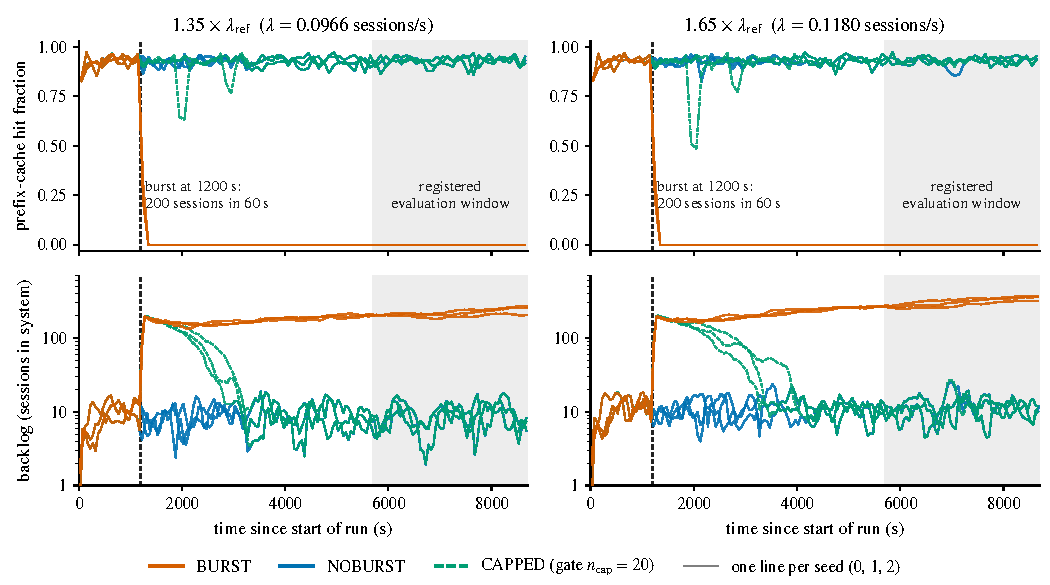
\includegraphics[width=\textwidth]{figs/fig1_e2_timeseries.pdf}
\caption{The registered paired test on SGLang (E2) at nominal rates of 1.35 $\lref$ (left) and 1.65 $\lref$ (right), $\lref=0.0715$\sps; over the evaluation window the three seeds delivered 1.27--1.45 and 1.61--1.75 $\lref$. Top: hit fraction (turns with more than half of the prompt cached) in 100\,s windows. Bottom: sessions in the system (log scale), including those in tool calls. One thin line per seed and arm. Dashed: a burst of 200 sessions at 1200\,s. Shaded: the registered evaluation window. The hit series is recomputed from the request logs and matches the registered per-run value to four decimals.}\label{fig:e2}
\end{figure*}

An LLM agent that uses tools sends its serving engine sessions of many turns. Each turn's prompt is the previous context plus the output of the tool just run, and between turns the session is idle while the tool runs. Prefix caching keeps the key--value (KV) state of the previous turn in GPU memory, so a follow-up turn whose prefix is still cached prefills only its new tokens~\citep{zheng2024sglang}. In our workload a follow-up turn that hits prefills 551 tokens, while a miss prefills the whole prompt, about 10,500 tokens on average; over a session, prefill work with every follow-up hitting is about 16 times smaller than with every turn missing.

We show that this can make the engine's good state, in which almost every follow-up turn hits, \emph{metastable}. Let $\lmiss$ be the all-miss capacity, the session throughput of a saturated engine when every turn misses, and $\lref$ its estimate from saturated runs with caching disabled (0.0715\sps{} on SGLang with a 300,000-token KV pool). In our measurements an empty server carried nominal arrival rates between 1.25 and 2 times its own $\lref$ for 3000\,s with 91--93\% of turns hitting, on SGLang and on vLLM with that pool, and up to 5.5 times $\lref$ when SGLang sized its own KV pool. Each rate is a single run with one arrival realization, whose realized rates were 6--13\% above nominal, except that on SGLang with the 300k pool three fresh arrival seeds were run at 2.0 and 2.5 $\lref$ and all stayed good, although the original seed had been unstable at 2.5; ordered by realized arrival rate, the 12 runs put that pool's edge between 2.67 and 2.73 $\lref$ (\S\ref{sec:edge}). A transient burst admits more sessions than the KV pool can hold once their contexts grow. A session with no running request, whether in a tool call or waiting in the queue, holds no lock on its KV, so admitting waiting work evicts it, oldest first; when its next turn is admitted it misses, the miss costs an order of magnitude more prefill, the queue grows, the gap between a session's turns grows with it, and more idle KV is evicted before its owner returns. Every turn then pays a full prefill, and the backlog does not drain (Fig.~\ref{fig:e2}).

Neither the collapse nor the loop that sustains it is new. Throughput that collapses when the working sets of the admitted jobs exceed memory is Denning's thrashing~\citep{denning1968thrashing,denning1968working}, and a bad state that a feedback loop sustains after its trigger is gone is a metastable failure~\citep{bronson2021metastable,huang2022metastable}. That KV left idle during tool calls is evicted and costly to recompute motivates Continuum, InferCept, MORI and TokenCake~\citep{li2025continuum,abhyankar2024infercept,xia2026mori,bian2025tokencake}, and Sutradhara observes, under Poisson load on vLLM, that prefix hit rates collapse despite context reuse, and attributes this to LRU eviction (as in vLLM and SGLang) of the contexts of requests waiting on tool calls~\citep{biswas2026sutradhara}; ThunderAgent and NVIDIA Dynamo treat agents' KV eviction and re-prefill as working-set thrashing~\citep{kang2026thunderagent,dhanani2026dynamo}, and EfficientAgent applies Denning's working-set principle and load control to the host KV tier of a fixed pool of agents~\citep{shao2026efficientagent}. The loop between eviction, cold prefill and queueing is published for closed or bounded populations: for RL rollouts under a concurrency ceiling, MISA-T reports vLLM Router's prefix-cache hit rate falling from 92.4\% to 4.5\%, describes the loop and interrupts it with a session cap~\citep{hong2026misat}; CONCUR halves its window of active agents when the hit rate falls below 0.2 while KV usage exceeds 0.5~\citep{chen2026concur}; Yuan et al.\ and VAMP measure the collapse on vLLM~\citep{yuan2026agentic,kim2026vamp}; and AgentKV, known to us from its abstract, predicts its onset at high concurrency from available KV capacity over per-instance context demand~\citep{anon2026agentkv}. Under open Poisson arrivals on vLLM, KAIROS reports thrashing when its controller lowers the GPU clock or when the arrival rate rises, and, in one run without its thrashing avoidance, a persistent thrashing regime at an arrival rate that a baseline at the maximum clock carries; that run shows no frequency trace, so whether its trigger was removed is not reported, and it has no burst trigger, no fixed clock, no replication and no matched arms~\citep{yuan2026kairos}. What we add is a controlled, replicated test at a fixed clock and pool, two persistent states at one capacity and one arrival rate, entered by a transient burst and checked against matched no-burst and capped arms on common random numbers, and a first-principles account of the thrashing curve in which the hit rate feeds back on itself through the service time and the KV held by running requests, and in which, on the memory-gated all-miss branch, the queue rather than the tool time sets the gap between a session's turns.

Under the default FCFS ordering, our model and simulator predict that a server that passes steady-state load tests at a rate above $\lmiss$ at which it stays good from empty is one sufficiently large burst away from a collapse that, once deep, it does not leave unless the arrival rate falls below $\lmiss$ or admission is bounded. On the engine we have tested two rates per pool with a burst of 200 sessions and, in the registered test B1 at 1.65 $\lref$ on the 300k pool, bursts of 25 and 100: 25 left the engine good and 100 trapped it, in 3 of 3 seeds each, so the good state has a finite basin whose boundary lies between 25 and 100 sessions (\S\ref{sec:frozen}). Registered tests of burst sizes in between, of a cap engaged inside an established trap, of a pause in arrivals and of a temporary slowdown of tool calls are listed there with their frozen predictions, and their outcomes are pending in this version. In our earlier simulator, TTL pins with their pinned-first order, under the preview's release rule, and a pure resident-first order (LPM without SGLang's 128-request fallback) raise the rate below which the system recovers (\S\ref{sec:mech}). On the engine, stock LPM recovered from a 200-session burst at 1.35 $\lref$ in 4 of 6 exploratory runs but in only 1 of 6 at 1.65 (\S\ref{sec:grid}); on our reading of its source, it stops re-sorting its queue when more than 128 requests wait, so in deep congestion Proposition~\ref{prop:A} applies to it as well. With that fallback disabled, in an exploratory run at 1.65 $\lref$, LPM did not collapse on the two arrival streams on which stock LPM had collapsed in 4 of 4 runs, but no run recovered by the registered rule (\S\ref{sec:mech}).

\paragraph{Claims.} Each item says what is ours and what is not; \S\ref{sec:related} gives the full positioning.
\begin{itemize}
\item \textbf{Registered open-system metastability on two engines} (\S\ref{sec:e2}--\ref{sec:vllm}). At a clock, pool and Poisson arrival rate that the engine carried in the good state for the full 8700\,s of every no-burst run, a burst of 200 sessions within 60\,s left it at zero hits, with a backlog that did not drain, to the end of the run, 7500\,s later, and a client-side cap at the peak of $\mu(n)$ drained the same burst. In two pre-registered SGLang tests (pools of 300,000 and 955,757 tokens) BURST was at zero hits in 12 of 12 runs and trapped by the registered rule in 11, NOBURST was good in 12 of 12 and CAPPED recovered in 12 of 12; on vLLM 0.32.0 the registered analysis of a third test passes at both rates, but the frozen decision rule for its mechanism checks is not met, because its online detector also alarmed, during the drain, in two capped runs (\S\ref{sec:vllm}). The loop was published for closed populations, and KAIROS reports a persistent thrashing regime under open arrivals in one uncontrolled run whose clock during the thrashing is not reported~\citep{yuan2026kairos}; ours is a controlled, replicated test at a fixed clock and pool, with a burst trigger and the trigger-and-control design of Huang et al.~\citep{huang2022metastable}: two persistent states at one capacity and offered load, against matched no-burst and capped arms on common random numbers, on two pools and two engines.
\item \textbf{The sustaining variable} (\S\ref{sec:mechanism}). At the same load, the ratio of the reuse gap to the pool's turnover time $R_M=M/\text{churn}$, the time in which the pool is rewritten, is 0.010--0.028 in every good-state run and 4.1--9.7 in every BURST run, on both engines and both pools; turn latency, not tool time, carries the gap past $R_M$, and the trapped value obeys a cost-model-free identity (Proposition~\ref{prop:trapid}). The miss criterion is Denning's and Che's~\citep{denning1968working,che2002hierarchical}, that queueing behind other agents lengthens the gap between an agent's turns has been measured for the host KV tier of a closed pool of agents, whose backlogged-pool working-set scale is the cycle argument behind the identity (EfficientAgent~\citep{shao2026efficientagent}), and the trap is an instance of what Huang et al.\ call capacity-degradation amplification; ours are the measurement in both states at one load and the identity's exact time-domain form on the all-miss FCFS branch, checked against the trapped runs with nothing fitted.
\item \textbf{A first-principles thrashing curve} (\S\ref{sec:fp}). We derive $\mu(n)$ from the pool size, the workload and an iteration-cost model fitted only to server-log timing, with no parameter fitted to any $\mu(n)$, hit or trap measurement (the H200 and vLLM cells take one speed factor fitted to their all-miss token rate), and prove, for the deterministic model, a closed-form all-miss onset (the sessions in tool calls plus one pool of running sessions), a speed law (a faster GPU moves the onset out and lowers the peak ratio $\mu^*/\lmiss$), a fold criterion (a proof sketch) and the trapped identity. The model reproduces the two SGLang curves and misses vLLM's earlier cliff. Metastability from a unimodal throughput curve and its cure by bounded admission are classical~\citep{kleinrock1975aloha,carleial1975bistable,courtois1975decomposability,nelson1987stochastic}, with the slowdown given as a function of occupancy; ours are the derivation of the curve and its closed forms.
\item \textbf{Frozen out-of-sample predictions} (\S\ref{sec:frozen}). Before their results were read by the agents that derived the model, we froze its predictions for an H200 at the same pool, for pools of 150,000 and 600,000 tokens, for Llama-3.1-8B, for a registered dose-response of the probability of a stuck run against burst size (critical fresh burst 53.4 sessions at 1.65 $\lref$) and for a registered rescue in which a cap engaged inside an established trap drains it and the good state persists after release. For the H200 the model predicted a peak ratio of 1.92 at $n\approx32.5$ (against 3.27 predicted and 3.15 measured on the A100), a 0.5-hit crossing at 37.3 sessions and a from-empty edge at 1.39 $\lref$; the engine gave 1.89 at $n=32$ (turns-based; 1.99 in completed sessions), a crossing near 38.9 and, on the original seed-0 runs, an edge in $[1.3,1.4)\,\lref$ (on reseeding, 1.4 $\lref$ was stable in seeds 1 and 2). Past the crossing the measured hit fraction fell gradually, to 0.46 at $n=40$ (0.27 predicted), 0.32 at 44 and 0.16 at 52, where the model is all-miss beyond its onset at 41.3 sessions, so the predicted onset came early; we have not traced this miss to a specific assumption (\S\ref{sec:fp-weak}). The first author, though not those agents, had seen the H200 closed-curve values for $n\le32$, which include the peak, so the H200 peak ratio is not blind to him. The registered basin test B1 passed as predicted: the model gave this exact outcome probability 0.879 (its 100-session predictions blind by access only, since those runs had ended before the push), and the simulator's calls matched all 6 of its runs and all 6 runs of a fresh-seed from-empty test, which did not replicate the first seed's edge (\S\ref{sec:frozen}). The other outcomes are pending in this version. That trap probability depends on the size of the trigger is part of metastability theory~\citep{bronson2021metastable,huang2022metastable,isaacs2025analyzing}; ours is a boundary on an LLM engine predicted before it is measured.
\item \textbf{An ordering bound} (\S\ref{sec:props}). Under request-level FCFS and the assumptions of \S\ref{sec:props}, no online eviction rule, queued-prefix protection and FCFS-order TTL pins included, lets $\mu(n)$ exceed the all-miss capacity as $n\to\infty$ if the congested engine computes prompt tokens no faster than with caching disabled; stock SGLang LPM falls under it in deep congestion through its 128-request fallback. The prefill-saturation bound is MISA-T's~\citep{hong2026misat}, and that arrival-order service sustains metastability is known~\citep{bronson2021metastable,farahbakhsh2026characterizing}; ours is that request-level FCFS drives reuse to zero in congestion whatever the online eviction rule, so that the bound becomes the all-miss capacity.
\item \textbf{A pre-deployment procedure, evaluated} (\S\ref{sec:diag}). Measure $\lmiss$ with the cache off, $\mu(n)$ across the cliff and the from-empty edge; cap admitted sessions at the smallest $n$ within 5\% of the peak, inside the interval $(n_1,n_2)$ of Corollary~\ref{cor:rescue}; re-measure for each workload, pool, engine and GPU. Multiprogramming-level selection, session-based admission, client-side concurrency limits and hit-rate thrashing signals are prior art~\citep{denning1976optimal,cherkasova2002session,maurer2015fail,chen2026concur,hong2026misat}; ours are the evaluation and the placement condition.
\end{itemize}
Registrations committed before their runs, with GitHub's push log as the external record of when each became public, and predictions frozen under pushed tags are how we tried to make these claims checkable. They are rigor, not a contribution; Appendices~\ref{app:prereg} and~\ref{app:timeline} list every registration and prediction round, with the slips in them.

The registered tests use one model, Qwen2.5-7B-Instruct, one GPU type, the A100 80GB, and synthetic sessions with exponential 5\,s tool times and no shared prefixes; on an H200 at the same pool the window narrowed from $(1,2.0)$ to $(1,1.3)$ times that GPU's own $\lref$, too narrow for our registration rule to place its two test points, so that cell is a measurement, not a registered test, and the Llama-3.1-8B cell of \S\ref{sec:frozen}, whose outcome is pending, extends the first. The vLLM registration was committed before its jobs were submitted but reached GitHub only after the first two had started, so we call that test registered, not pre-registered, and its BURST arm reuses the seeds of earlier exploratory vLLM runs (\S\ref{sec:vllm}).
